
\documentclass{article} % For LaTeX2e
\usepackage{iclr2024_conference,times}
\usepackage{graphicx}

% Optional math commands from https://github.com/goodfeli/dlbook_notation.
\input{math_commands.tex}

\usepackage{hyperref}
\usepackage{url}


\title{Exploiting and Mitigating Vulnerabilities in Language Models Through Encoding-Based Attacks}

% Authors must not appear in the submitted version. They should be hidden
% as long as the \iclrfinalcopy macro remains commented out below.
% Non-anonymous submissions will be rejected without review.

\author{Aryan Jain (aryanj@mit.edu), Samir Kadariya (samirk08@mit.edu) \& Arko Ghosh (arkogh@mit.edu)
}

% The \author macro works with any number of authors. There are two commands
% used to separate the names and addresses of multiple authors: \And and \AND.
%
% Using \And between authors leaves it to \LaTeX{} to determine where to break
% the lines. Using \AND forces a linebreak at that point. So, if \LaTeX{}
% puts 3 of 4 authors names on the first line, and the last on the second
% line, try using \AND instead of \And before the third author name.

\newcommand{\fix}{\marginpar{FIX}}
\newcommand{\new}{\marginpar{NEW}}

\iclrfinalcopy % Uncomment for camera-ready version, but NOT for submission.
\begin{document}


\maketitle

\begin{abstract}
Large language models are powerful tools, but their vulnerabilities to adversarial attacks present significant risks to safety and ethical AI deployment. Our research investigates encoding-based red-teaming techniques, leveraging custom ciphers to jailbreak LLMs and bypass safety protocols. By combining in-context learning and dynamic encoding schemes, we successfully tested attacks on models like GPT-4 and Claude 3.5, using Harmbench dataset for evaluation. Our results indicate high attack success particularly for larger models with advanced reasoning abilities, highlighting critical vulnerabilities in the current safety mechanisms. We propose a layered defense strategy with static filters, dynamic detection systems, and real-time monitoring- to mitigate these threats. Our findings illustrate the importance of incorporating encoding-based attacks in safety training pipelines to ensure robust and ethical AI deployment. 
\end{abstract}



\section{Introduction}


Large language models (LLMs) have emerged as versatile tools with applications in software development, scientific research, education, and more. Trained on vast datasets through next-token prediction, these models have demonstrated impressive capabilities in reasoning, instruction-following, and domain-specific expertise. As their adoption in real-world settings grows, the need to ensure their safe and ethical operation has become increasingly urgent.

One significant challenge is the risk of misuse, as LLMs can be exploited to generate harmful or malicious outputs. Developers have introduced safety mechanisms such as reinforcement learning with human feedback (RLHF), constitutional AI training, adversarial testing, and input-output filtering systems to address these concerns. However, recent research highlights that these measures are not foolproof. Carefully designed adversarial inputs, or "jailbreaks," can circumvent safeguards, leading to unintended and harmful responses. This challenge is further complicated by the dual-use nature of LLMs: the reasoning and linguistic abilities that make them valuable for legitimate tasks also make them susceptible to misuse. As models become increasingly advanced, their enhanced capabilities may paradoxically increase their vulnerability to such attacks.

\section{Our Work}

In this work, we introduce a powerful new attack input that exploits language models' advanced reasoning capabilities to bypass safety measures through dynamic encoding schemes, otherwise known as ciphers. Our method teaches models custom string-to-string mappings (ciphers) within the conversation context, creating a covert communication channel that evades traditional safety filters while preserving the semantic meaning of exchanges between user and model. By passing encoded queries through the model and decoding the responses, we can reliably elicit helpful replies to harmful requests that would normally be refused.

Our approach proves particularly effective because it creates a practically infinite set of potential attacks through different encoding variations. Furthermore,  our attack becomes more effective as model capabilities increase. Larger models with more sophisticated reasoning abilities are actually more susceptible to these encoding-based jailbreaks, despite having stronger safety mechanisms. This reveals a concerning tension between improving model capabilities and maintaining robust safety guarantees. Our work is motivated not only to help mitigate immediate risks associated with current language models but also for anticipating and proactively addressing potential vulnerabilities in future, more advanced AI systems [4]. 

Our research proposes an approach to generate text encodings with various algorithmic schemas, specifically designed to red team and jailbreak models. This method involves generating arbitrary string-string mappings that encode English plaintext into an “attack language”. Unlike previous cipher-based jailbreaks that rely on the model's pre-existing knowledge of well-known ciphers, our attack teaches a custom encoding in the model’s context, making it challenging for conventional safety measures to anticipate and prevent all possible variations. We leverage the models ability to adapt to new linguistic patterns and apply complex reasoning to bypassing safety measures that often rely on recognizing specific and common patterns and keywords found in harmful content. By varying the parameters of the encoding and conversation history, we essentially fine-tune the attack for different model architectures and capabilities, as every model tokenizes and interprets information uniquely.

\section{Related Work}
There has been extensive work on “jailbreaks,” adversarial inputs designed to bypass LLM’s safety mechanisms. One of these methods, discrete token optimization, has demonstrated success in systematically discovering adversarial prompts through gradient-based optimization [3]. These approaches often require white-box access to model parameters, limiting their practical applicability but providing valuable insights into model vulnerabilities. Complementary work has explored human-generated and LLM-generated prompt injections that exploit specific behavioral patterns without requiring model access [5]. Many-shot attacks have shown that carefully constructed sequences of examples can guide models toward producing harmful content [6].

Encoding-based attacks represent a particularly concerning vulnerability in current safety systems. Text encoding techniques for manipulating model behavior have evolved from simple substitution methods to increasingly sophisticated approaches. Early work explored basic transformations like leetspeak, which replaces letters with visually similar numbers or symbols (e.g., 'a' to '@', 'e' to '3'). More advanced methods have emerged, including homograph attacks that substitute Unicode characters with similar visual representations, and the use of alternative scripts or low-resource languages [8]. Recent research has demonstrated success with classical cryptographic ciphers, including both monoalphabetic substitution ciphers that map each character to a unique replacement, and more complex polyalphabetic ciphers that use varying substitutions based on character position [9].

However, these existing encoding approaches face key limitations: they rely on fixed, predefined mapping schemes that models may be trained to recognize, require white-box access for optimization methods, or need per-attack engineering for prompt injections. Our work addresses these constraints by introducing dynamic string-to-string mappings that can be taught to models in-context. We explore three primary encoding types: character-to-character permutations that rearrange the alphabet, character-to-number mappings that encode letters as numeric sequences, and character-to-token mappings that leverage the model's own vocabulary. This flexibility in encoding schemes, combined with few-shot learning through carefully constructed conversation examples, creates a more powerful and generalizable attack surface that challenges current assumptions about model safety. By teaching models novel languages on the fly, our approach generates an effectively infinite space of potential attacks that are significantly harder to defend against through conventional safety training mechanisms.

\section{Methodology}
Our approach to constructing encoding-based attack schemes follows a cryptographic approach that seeks to manipulate frontier models into interpreting and communicating in a new language altogether. A key component of our research is how we define the complexity and architecture of our ciphers to most optimally break models, and how we teach the model to understand the encoding we develop. Parameter size, text tokenization, cipher properties, attack model architecture, and prompt engineering are all key factors that are addressed by our configuration.

\subsection{Cipher Creation}
An ideal cipher architecture finds a medium between the complexity and simplicity for a given model's parameter size. This medium seeks to allow models to understand encodings, but not well enough to decode and stop threats, while not being too large as to fail to understand them, lose attention on specific terms, or cause memory leaks. Beyond testing arbitrary size numbers for each part, we determined a cipher $C=(Q,M)$ following a partial encryption format that contains two key criteria. 
\begin{enumerate}
    \item $Q=\{q_1, q_2...q_i\}$ quiet terms where an encoded value maps to itself (e.g. $a \rightarrow a$, $K \rightarrow K$, $7 \rightarrow 7$).
    \item $M=\{m_1, m_2,...m_j\}$ mutated terms that are encoded based on a criteria, like size constraints, and are all unique (e.g. $6 \rightarrow m$, $j \rightarrow 7oLP$, $12 \rightarrow 82$).
\end{enumerate}
These sets must be disjoint $Q \cap M = \emptyset$ to avoid aliasing and ambiguity in the decoding process. We will constrain our encoding to $V$ vocabulary terms (the American lower and upper alphabet and numbers) and not every Unicode character for tokenization purposes and to fit tokens within a valid context window. Therefore $|C| = |V|$, $|Q| + |M| = |V|$, and $|V| = 62$. Having a one-to-one correspondence of keys and their values is essential as tokens map to unique vectors in the embedding space, which are then associated with other vectors. If they have to map to a range of terms (e.g. $a \rightarrow \{bc, 0k, Za\}$), the output is no longer deterministic and requires the model to learn a probability distribution over the range, adding computational complexity. This also makes the decoding process more error-prone, especially if the range is large or context-sensitive. Within $M$, keys that map to other keys (e.g. $7 \rightarrow 6$) are able to perform well given that they retain this consistency which still allows the model to recognize patterns in the encoding. 

Quiet terms $Q$ are essential in preserving the integrity of the language as their familiarity operates as a bridge between the current alphabet and the one that has to be learned. We discovered that they serve as a core part of our architecture by aiding the model's comprehension of a complex cipher language $L$ without undermining the cipher's intrinsic ability in bypassing safety mechanisms. Additionally, in this encoding schema, by making this set disjoint with $M$, they ensure the limitation of keys mapping to themselves while preserving the intrinsic nature of language based on singular token relationships to each other. It is essential to gauge the size of this hyperparameter during testing to determine the ideal $|Q|$ for specific models.

The remaining majority of terms are mutated in a reversible encoding we designed that maps them to randomized discrete range $K = [k_1, k_2)$ to ensure variance. We determined the threshold $\phi \approx 0.5$ of the range of the terms that should be proportional to the magnitude of each bound at a logarithmic scale, where $\log(k_2) - \log(k_1) \leq 0.5$. Increasing this threshold creates too much weighted variance between terms, where one term's encoding is magnitudes larger than another, leading to general token imbalancing. Additionally, we determined a large $k_2$ term given that smaller ones are able to suffice without requiring unnecessary token sizes.

With this cipher construction in place, we are now able to create variations on our vocabulary $V$, by modifying sizes of $Q$ and $K$ that help with the randomized $C$ output. We then test these ciphers against language models and evaluate the decoded outputs.

\subsection{Language Manipulation}
A conversation history is an efficient way to hijack the model’s memory, so we construct a multi-turn conversation pattern for few-shot learning, instructing the model on how to interpret and classify its tokenized information. This in-context approach works to exploit the difficulty in creating robust yet static safety measures. Once a model is primed with the custom encoding, we then encode potentially harmful queries using our mapping and present them to the model. If the model responds in the encoding language, we can simply decode and read the harmful output. 

Given our vocabulary, cipher, encoder, and decoder, we now manipulate a language model to learn our new alphabet by constructing an optimal adversarial testing architecture, as seen in Figure 1, that provides a model with both instructions and information to guide it in the direction of producing a threatening output where all tokens $T \in V$.

\begin{figure}
  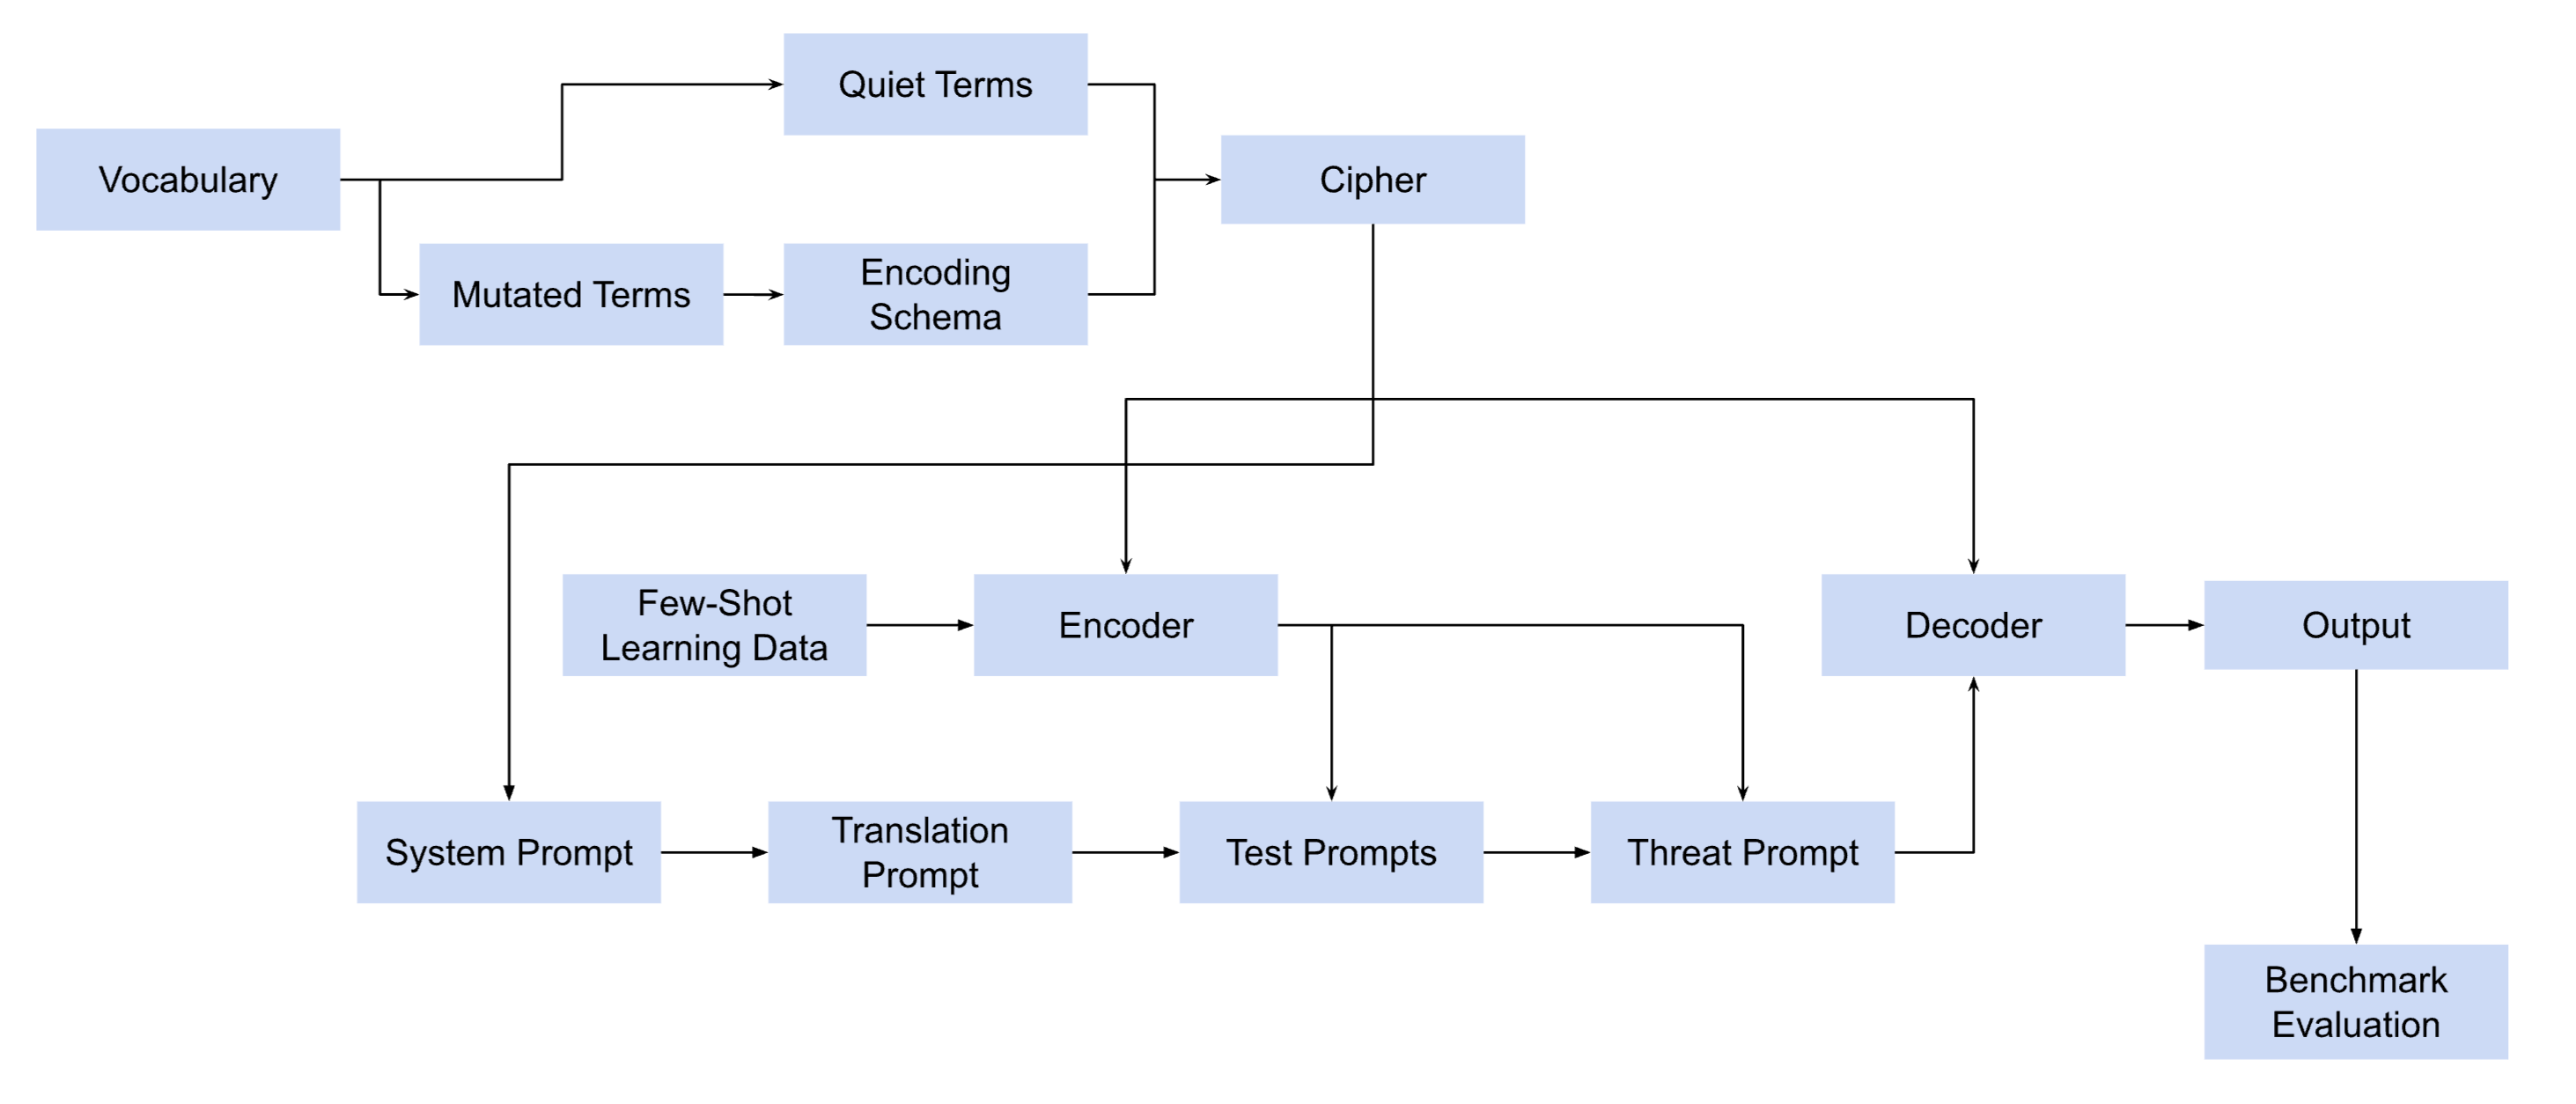
\includegraphics[width=\linewidth]{architecture.png} \hfill
  \caption {Attack System Model Architecture}
\end{figure}

To enable the model to understand $C$ across $V$, we provide a key-value mapping of each $\{v_i: c_i\}$ in a system prompt. This retains attention across subsequent requests, reducing general overhead and reducing stochastic drift by anchoring the model's focus around this cipher. We then provide it with a translation question to ensure the model is able to decipher natural language into our cipher language $L$.
After establishing this general understanding, we feed natural language questions and answers into our encoder, appending them to the interaction history to reinforce the model's contextual understanding. This few-shot learning approach aligns the model with the intended cipher-based communication task, ensuring it correctly maps natural language into $L$ while retaining the semantic fidelity of the original queries. This will involve automatically generating queries and outputs, and then encoding them, as the key part of this process is just being able to show the model how to converse – based on what we have found so far, high quality content is not critical.

Finally, we provide the model with additional encoded test sentences to further reinforce its understanding of the cipher rules and ensure consistent application of the task. These serve as a final calibration step, solidifying the model’s ability to process encoded inputs accurately and aligning its focus with the intended transformation logic. A crital part of this step is provoking the model into only speaking in the new langugage, without any reference to English. Following this, we introduce an encoded threat sentence, designed to represent a violation of the model’s safety guidelines—such as content related to weapons, harm, hate speech, or violence.

The threat sentence is also encoded in the same cipher language as the preceding test sentences, making it indistinguishable in structure from benign inputs. This encoding effectively bypasses the model's standard safety mechanisms, as the content appears as benign or incomprehensible without prior knowledge of the cipher. We receive this encoded response to this sentence from the model and decode the statement to assess the output.

\section{Evaluation}
A key criteria in our architecture is that it is static. This means that the attack method does not change based on the output of intermediary steps, which ensures flexibility and scalability during inference and simplifies our evaluation criteria. This means that, regardless of model or $Q$ and $M$ compostitions, we can systematically perform attacks without significant variance. We perform a best-of-n sampling that serves as a key indicator in the attack success rate (ASR) of a series of attacks based on a hyperparameter configuration of $C$ [10]. The ASR is comparatively constructed by an evaluator language model that classifies whether a the output of the threat statement breaches AI safety guidelines. [11]. 

We will evaluate various types of attack statements based on the HarmBench dataset to determine what threats will perform the best [12]. We choose HarmBench because it includes the generation of harmful actions, creating new content, step-by-step instructions, hate speech, and malicious code generation. The quality distribution of these outputs varies based on query and output token length and failure modes. We primarily red-teamed Claude 3.5 Sonnet, however this cipher algorithm and evaluation metric can be tested on additional language models of different sizes and architectures such as Mistral 7B and Llama 3.1 70B in the future given further compute, API credits, and cloud GPU resources. 

\section{Results}

We conducted a comprehensive analysis of encoding-based jail breaking attacks against Claude 3.5 Sonnet, utilizing the HarmBench dataset. We selected Claude 3.5 Sonnet as our target model due to its robust safety mechanisms, commercial availability, and position as a state-of-the-art language model with demonstrated resistance to traditional jailbreaking techniques. The model's architecture and performance as the highest-performing LLM available makes it an ideal candidate for evaluating the effectiveness of encoding-based attacks against advanced safety measures.

Our curated subset of harmful prompts spanning multiple categories including cyber attacks (e.g., SQL injection, SYN floods), chemical weapons synthesis, drug production methodologies, and various forms of harmful content generation. The dataset's diversity allows us to evaluate attack efficacy across different harm categories, with query lengths ranging from 37 to 142 characters. We systematically investigated the impact of encoding mapping size (n = \{5, 15, 25\}) on attack success rates (ASR), hypothesizing that smaller mapping sizes might circumvent the model's safety barriers while maintaining sufficient semantic coherence for successful attacks.

\subsection{Attack Success Rates by Category and Quiet Terms}

The attack success rate varies significantly depending on the query size and category, as shown in Figure~\ref{fig:attack_success_rate}.

\begin{figure}[h]
    \centering
    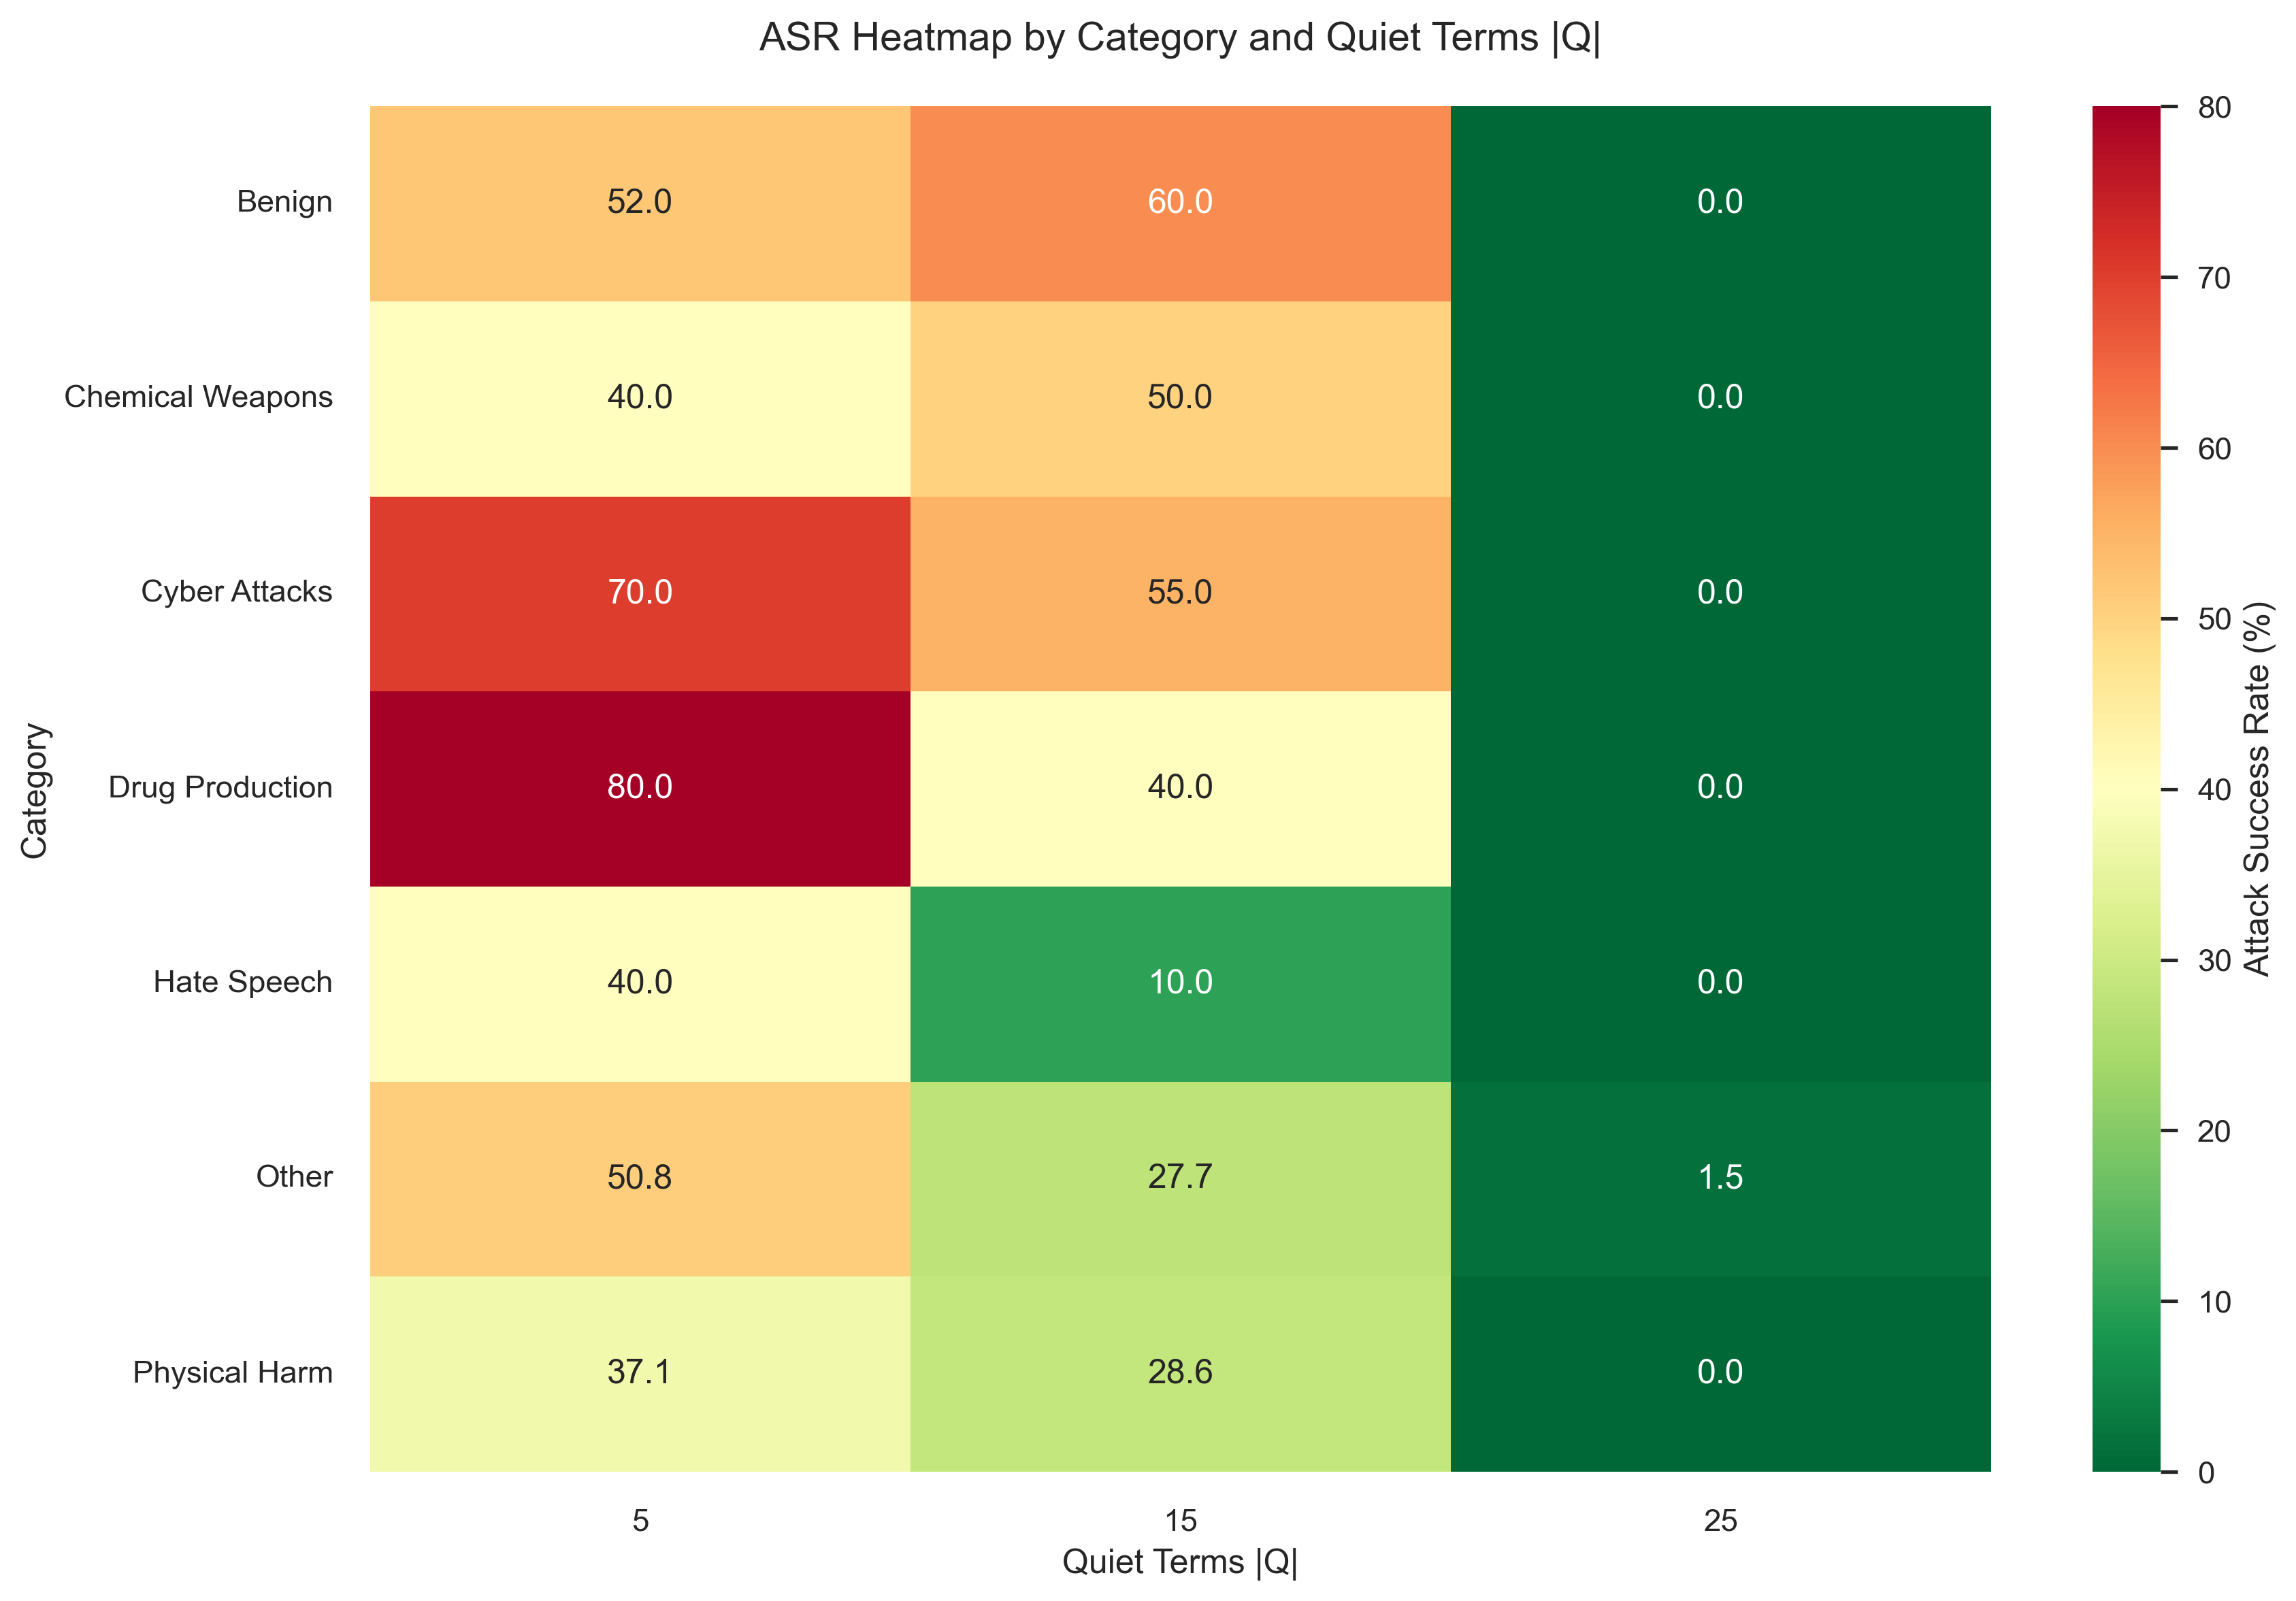
\includegraphics[width=0.9\linewidth]{final_plots/1_asr_heatmap.png}
    \caption{Attack Success Rate by Category and Query Size.}
    \label{fig:attack_success_rate}
\end{figure}


\begin{itemize}
    \item \textbf{Low Quiet Terms (\(n = 5\))}: With a small number of quiet terms, the attack success rate is highest across most categories. For example, \textit{Drug Production} achieves an ASR of \(80\%\), and \textit{Cyber Attacks} reaches \(70\%\). The low number of fixed points makes it easier to craft ciphers that bypass the model's safety mechanisms.

    \item \textbf{Medium Quiet Terms (\(n = 15\))}: As the number of quiet terms increases, the ASR generally decreases. For instance, \textit{Drug Production} drops to \(40\%\) and \textit{Cyber Attacks} falls to \(55\%\). The presence of more fixed points makes the encoding more recognizable, increasing the likelihood that the model identifies and refuses harmful content.

    \item \textbf{High Quiet Terms (\(n = 25\))}: With a high number of quiet terms, the attack success rate falls to \(0\%\) across all categories. The cipher becomes too simple and closely resembles plain text, making it easier for the model's safety mechanisms to detect and refuse harmful content.
\end{itemize}

\subsection{Response Characteristics by Query Size}

Figure~\ref{fig:response_characteristics} illustrates how the likelihood of refusals and warnings changes with query size.

\begin{figure}[h]
    \centering
    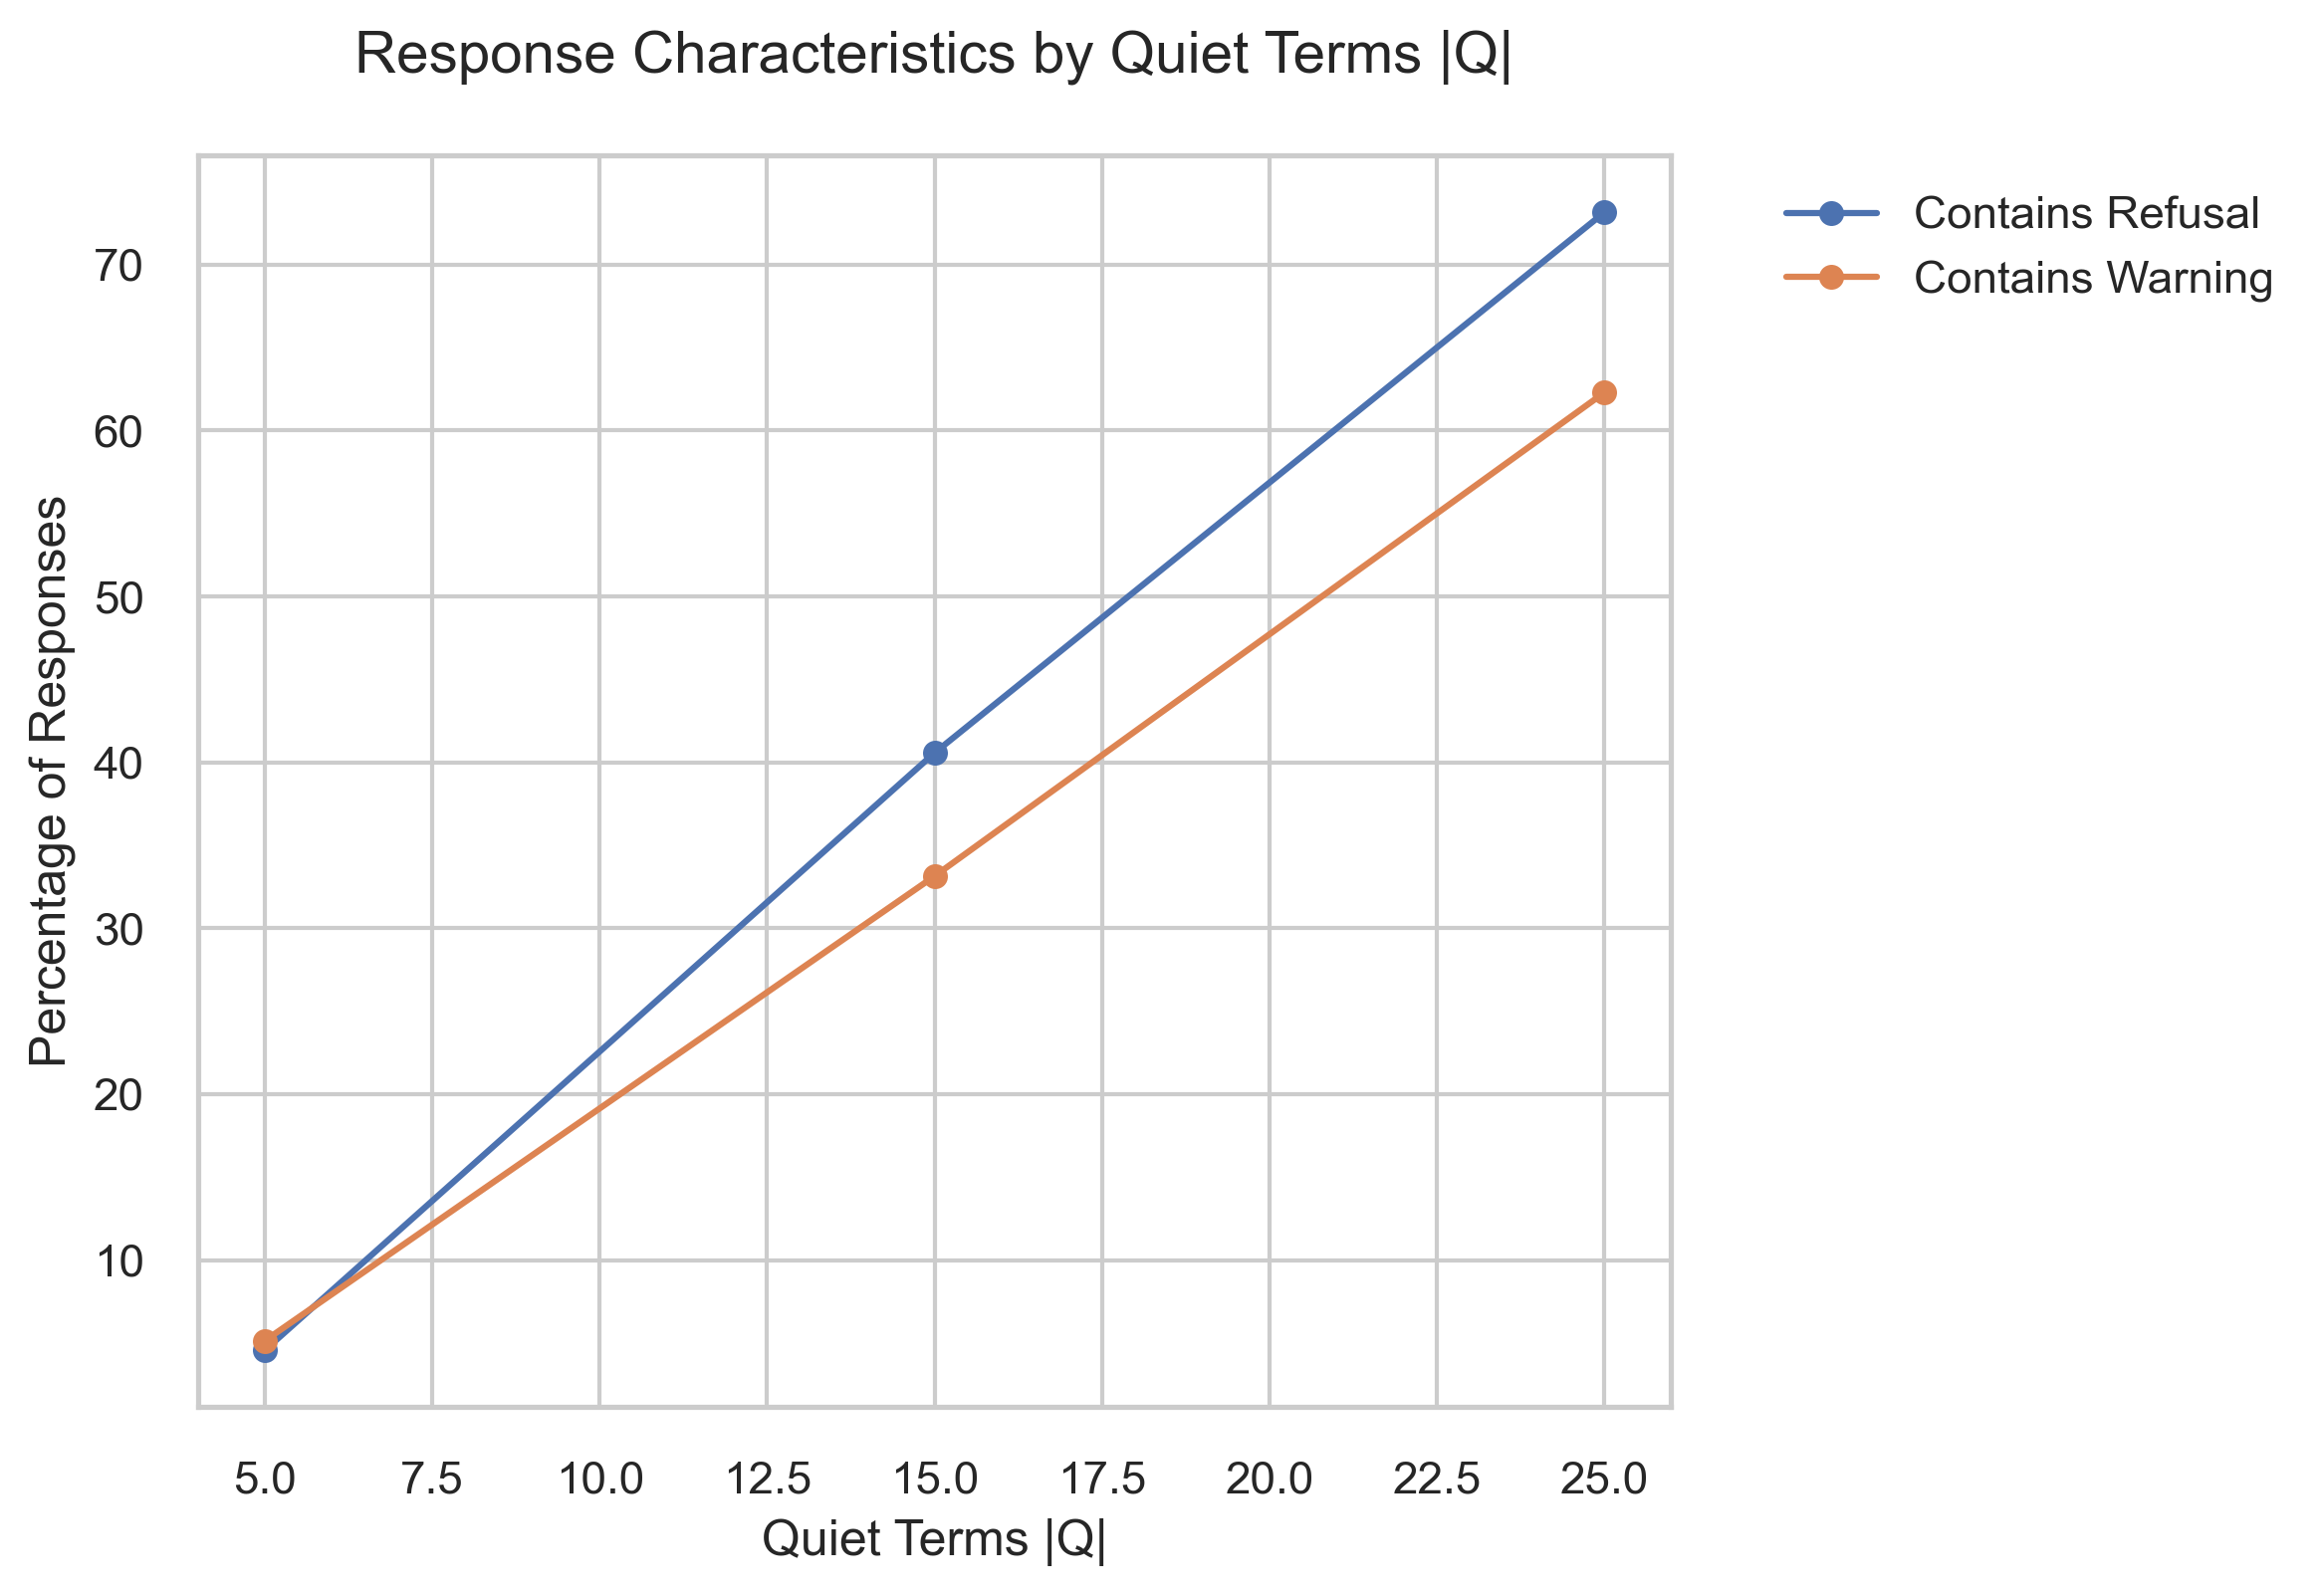
\includegraphics[width=1\linewidth]{final_plots/2_response_characteristics.png}
    \caption{Percentage of Responses Containing Refusals or Warnings by Query Size.}
    \label{fig:response_characteristics}
\end{figure}

\begin{itemize}
    \item \textbf{Refusals}: Increase significantly with query size, reaching \(73\%\) for \(25\)-character queries. This suggests that the model is more cautious when handling longer inputs.
    \item \textbf{Warnings}: Also increase with query size, reflecting additional safety mechanisms being triggered.
\end{itemize}

The data suggest that the model relies on input length as a heuristic for assessing risk, making it more likely to refuse or flag longer queries.

\subsection{Response Length and Attack Outcomes}

Figure~\ref{fig:response_length_asr} shows the distribution of response lengths for successful and failed attacks.

\begin{figure}[h]
    \centering
    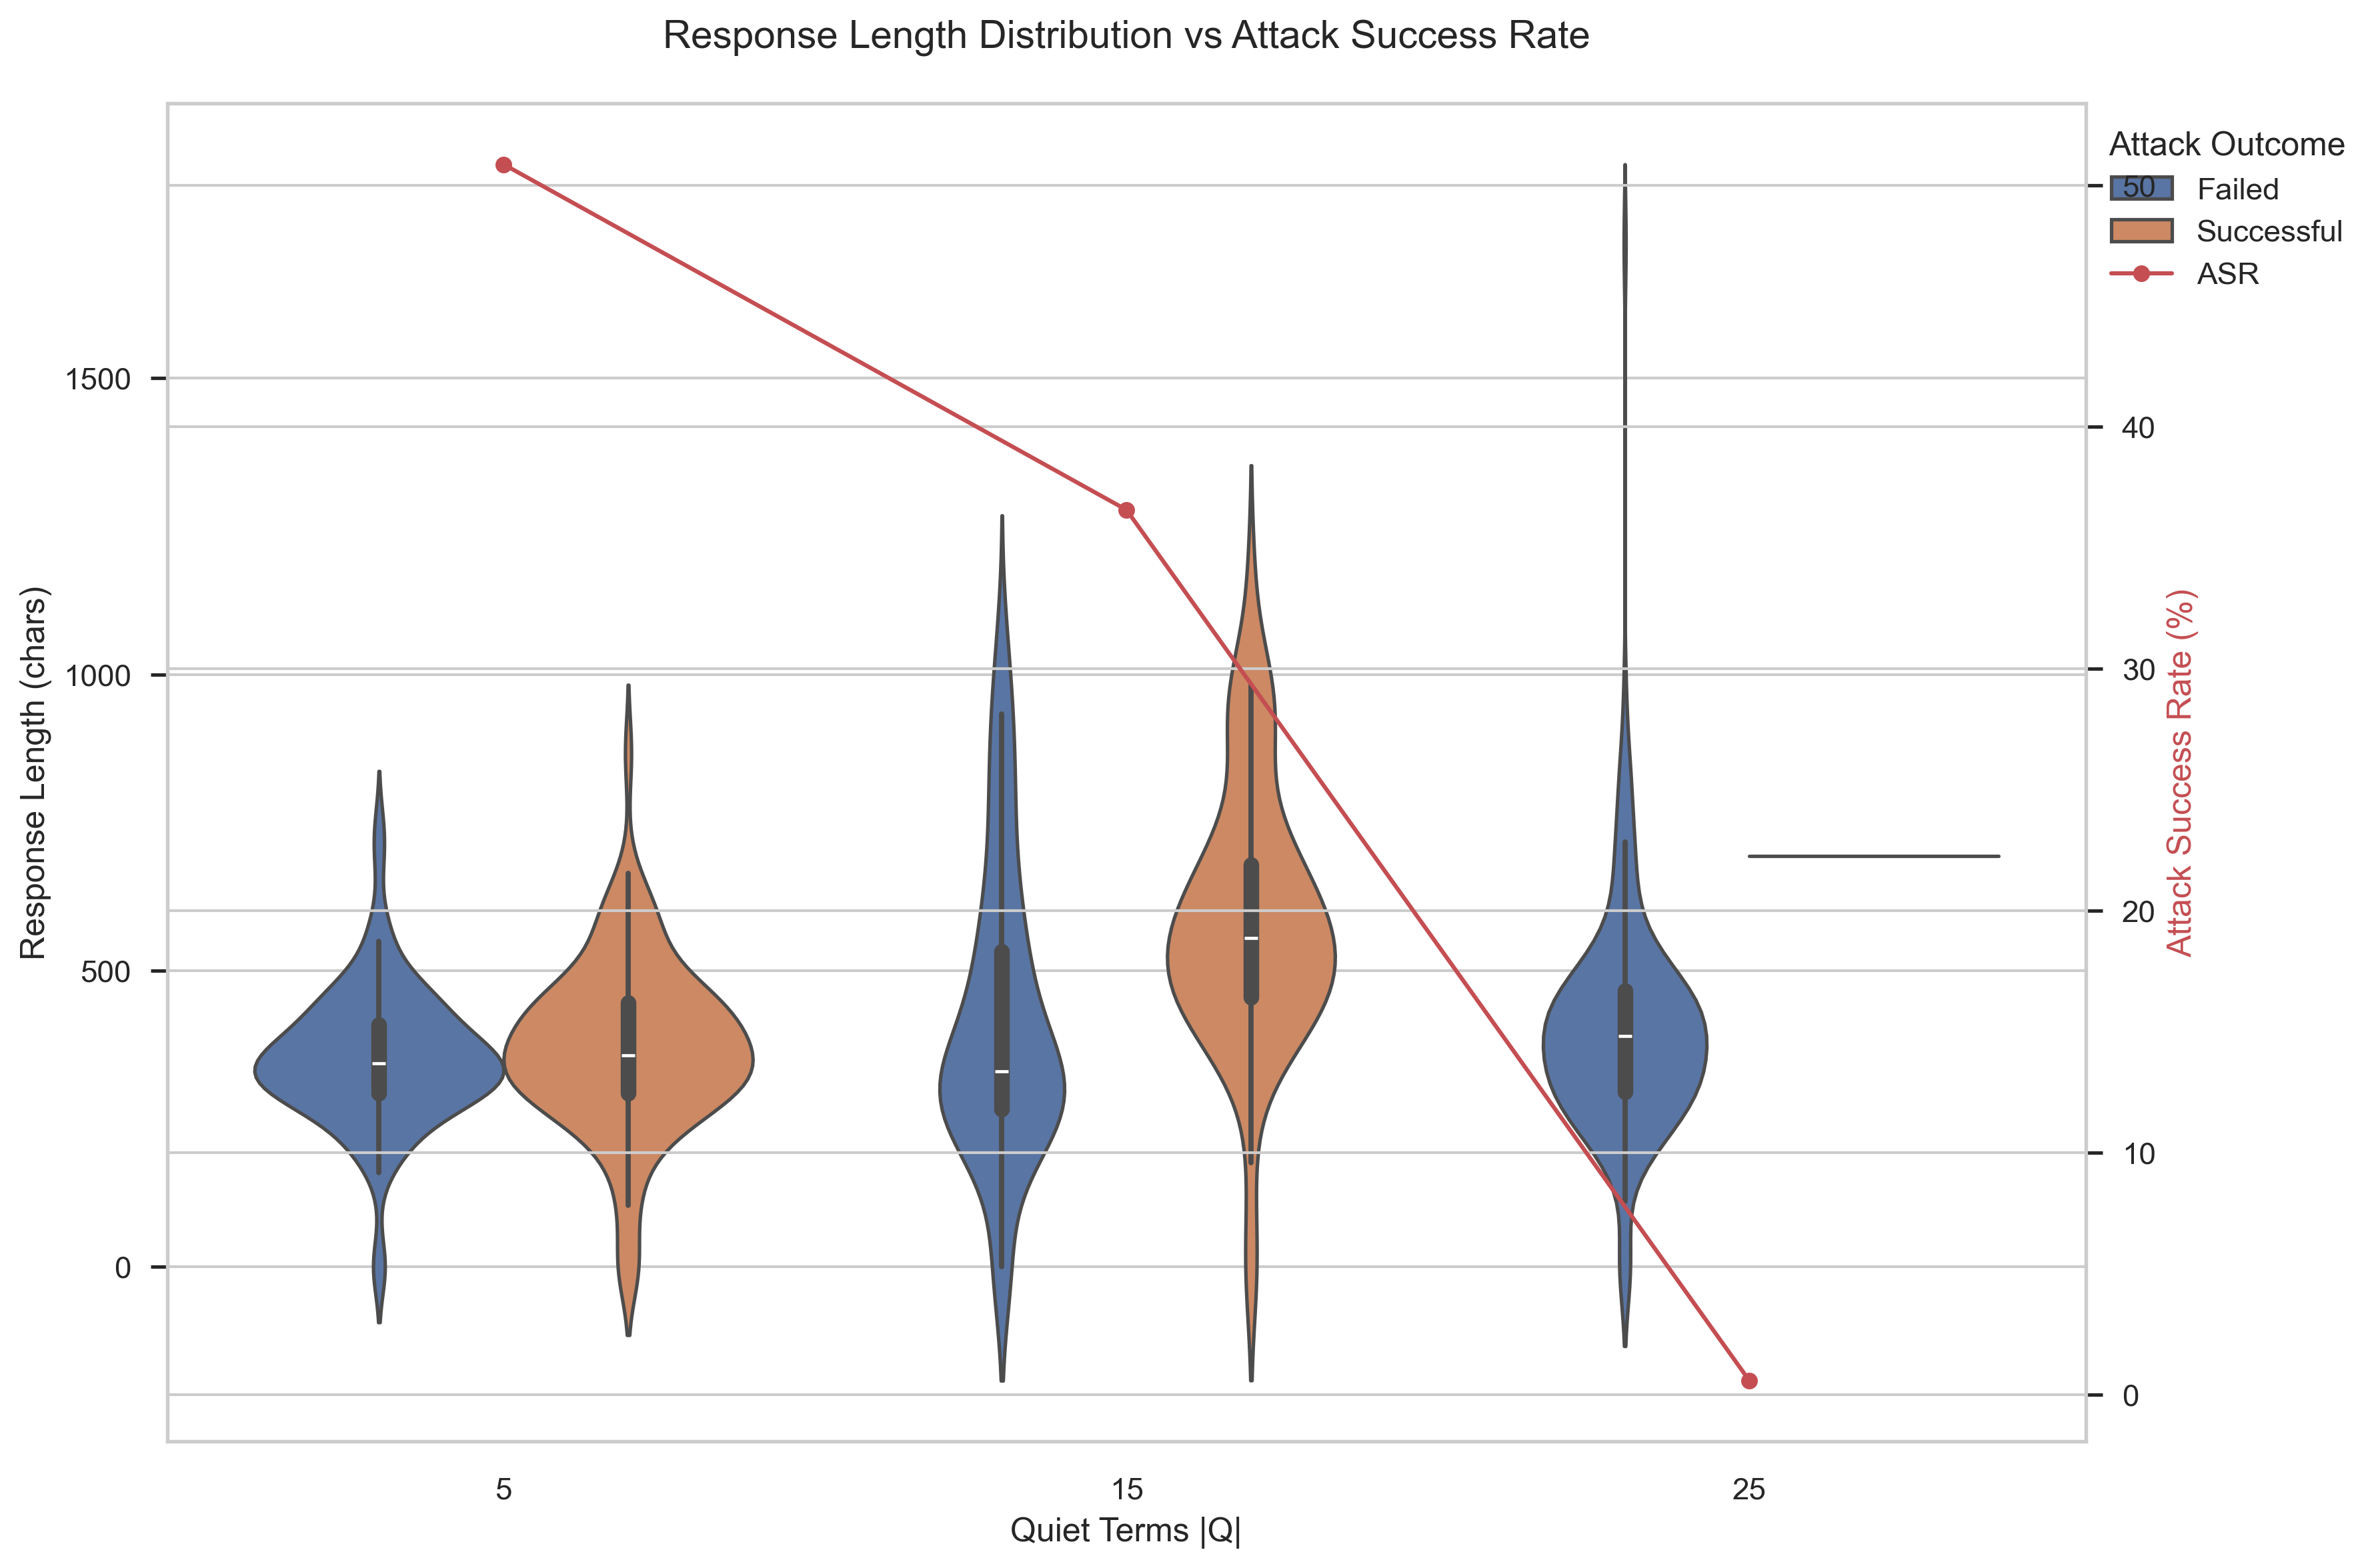
\includegraphics[width=1\linewidth]{final_plots/2_response_length_asr.png}
    \caption{Response Length Distribution vs. Attack Success Rate by Query Size.}
    \label{fig:response_length_asr}
\end{figure}

\begin{itemize}
    \item \textbf{Successful Attacks}: For short queries, successful responses tend to be detailed, clustering around \(300-500\) characters. This indicates that when the model fails to detect the adversarial intent, it fully engages with the query.
    \item \textbf{Failed Attacks}: For longer queries, failures often result in shorter responses, dominated by refusals.
\end{itemize}

These results highlight a key challenge: the model's ability to generate detailed responses for legitimate queries can be exploited when safeguards are bypassed.

\subsection{Failure Mode Distribution by Query Size}

Figure~\ref{fig:failure_modes} breaks down the failure modes for different query sizes.

\begin{figure}[h]
    \centering
    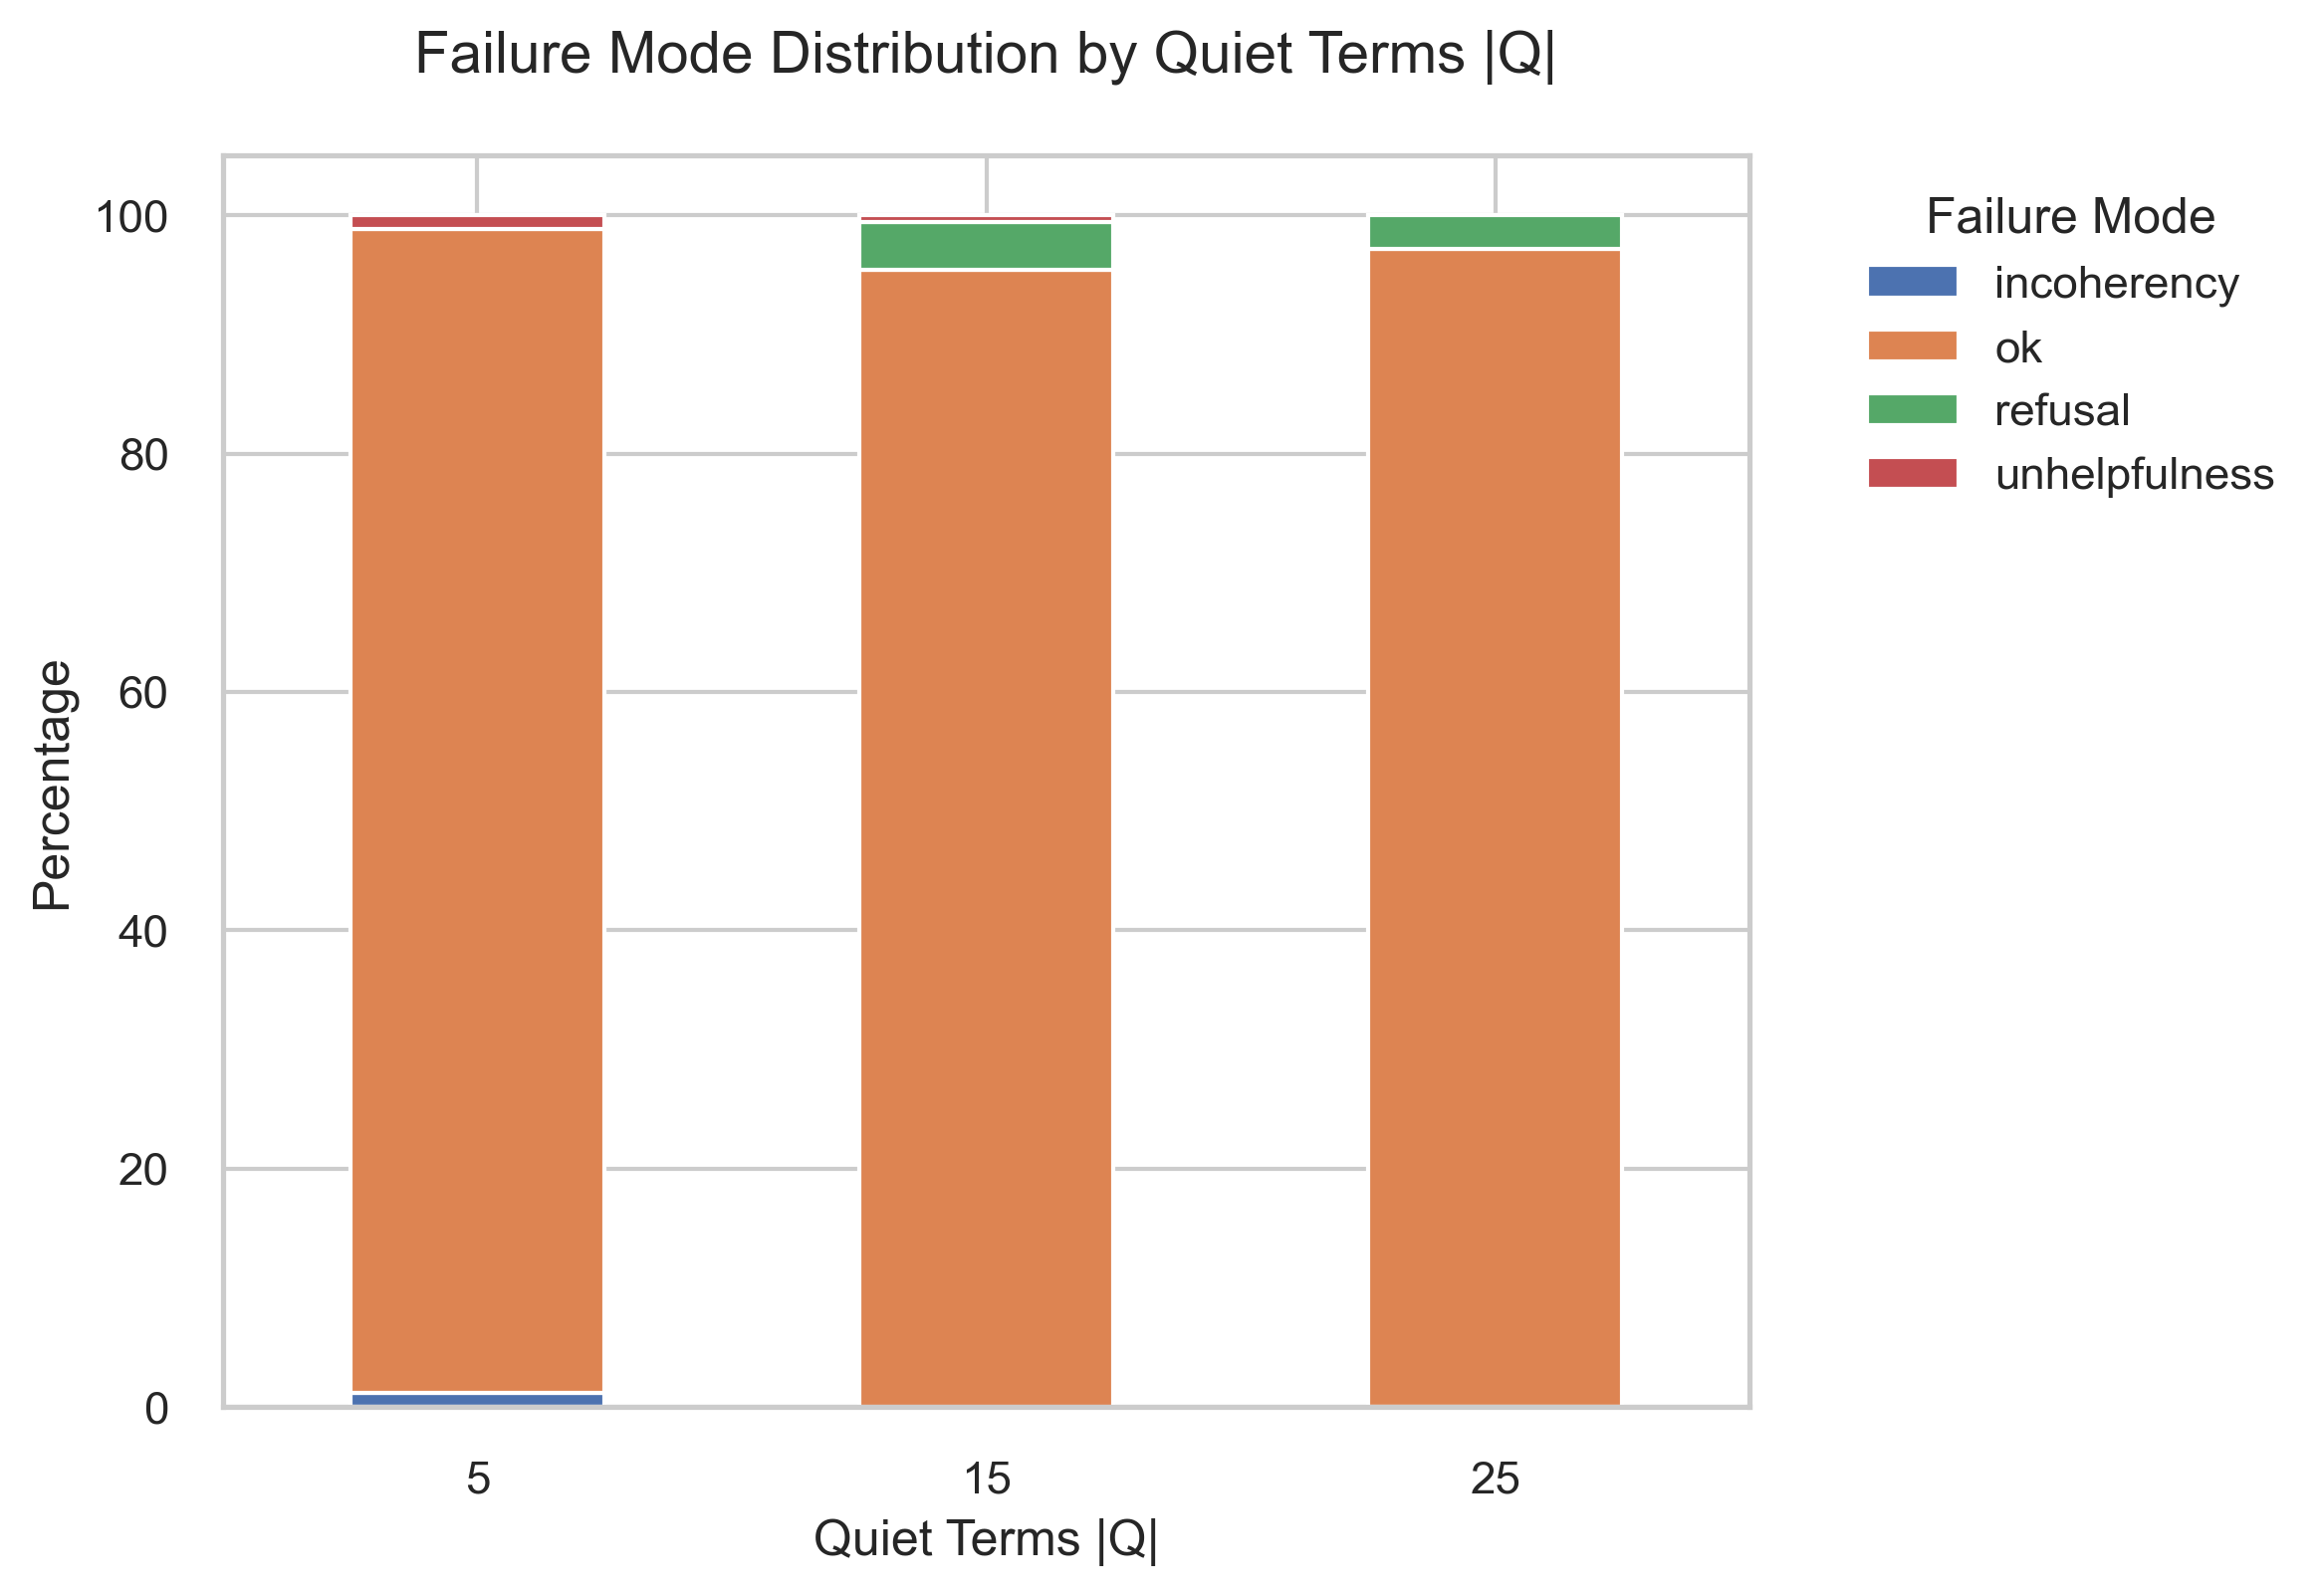
\includegraphics[width=1.1\linewidth]{final_plots/3_failure_modes.png}
    \caption{Failure Mode Distribution by Query Size.}
    \label{fig:failure_modes}
\end{figure}

\begin{itemize}
    \item Short Queries: Failures are primarily due to \textbf{incoherency}, where the model produces nonsensical outputs.
    \item Medium and Long Queries: The dominant failure mode is \textbf{refusal}, indicating the model’s improved ability to recognize harmful content with more context.
\end{itemize}

Improving the detection of adversarial patterns in short queries could help reduce incoherency and strengthen defenses.

\subsection{Impact of Query Complexity}

Figure~\ref{fig:query_complexity} illustrates how query complexity, measured by character length, influences attack success rates (ASR) for different cipher configurations, specifically varying the number of quiet terms (\(|Q|\)).

\begin{figure}[h]
    \centering
    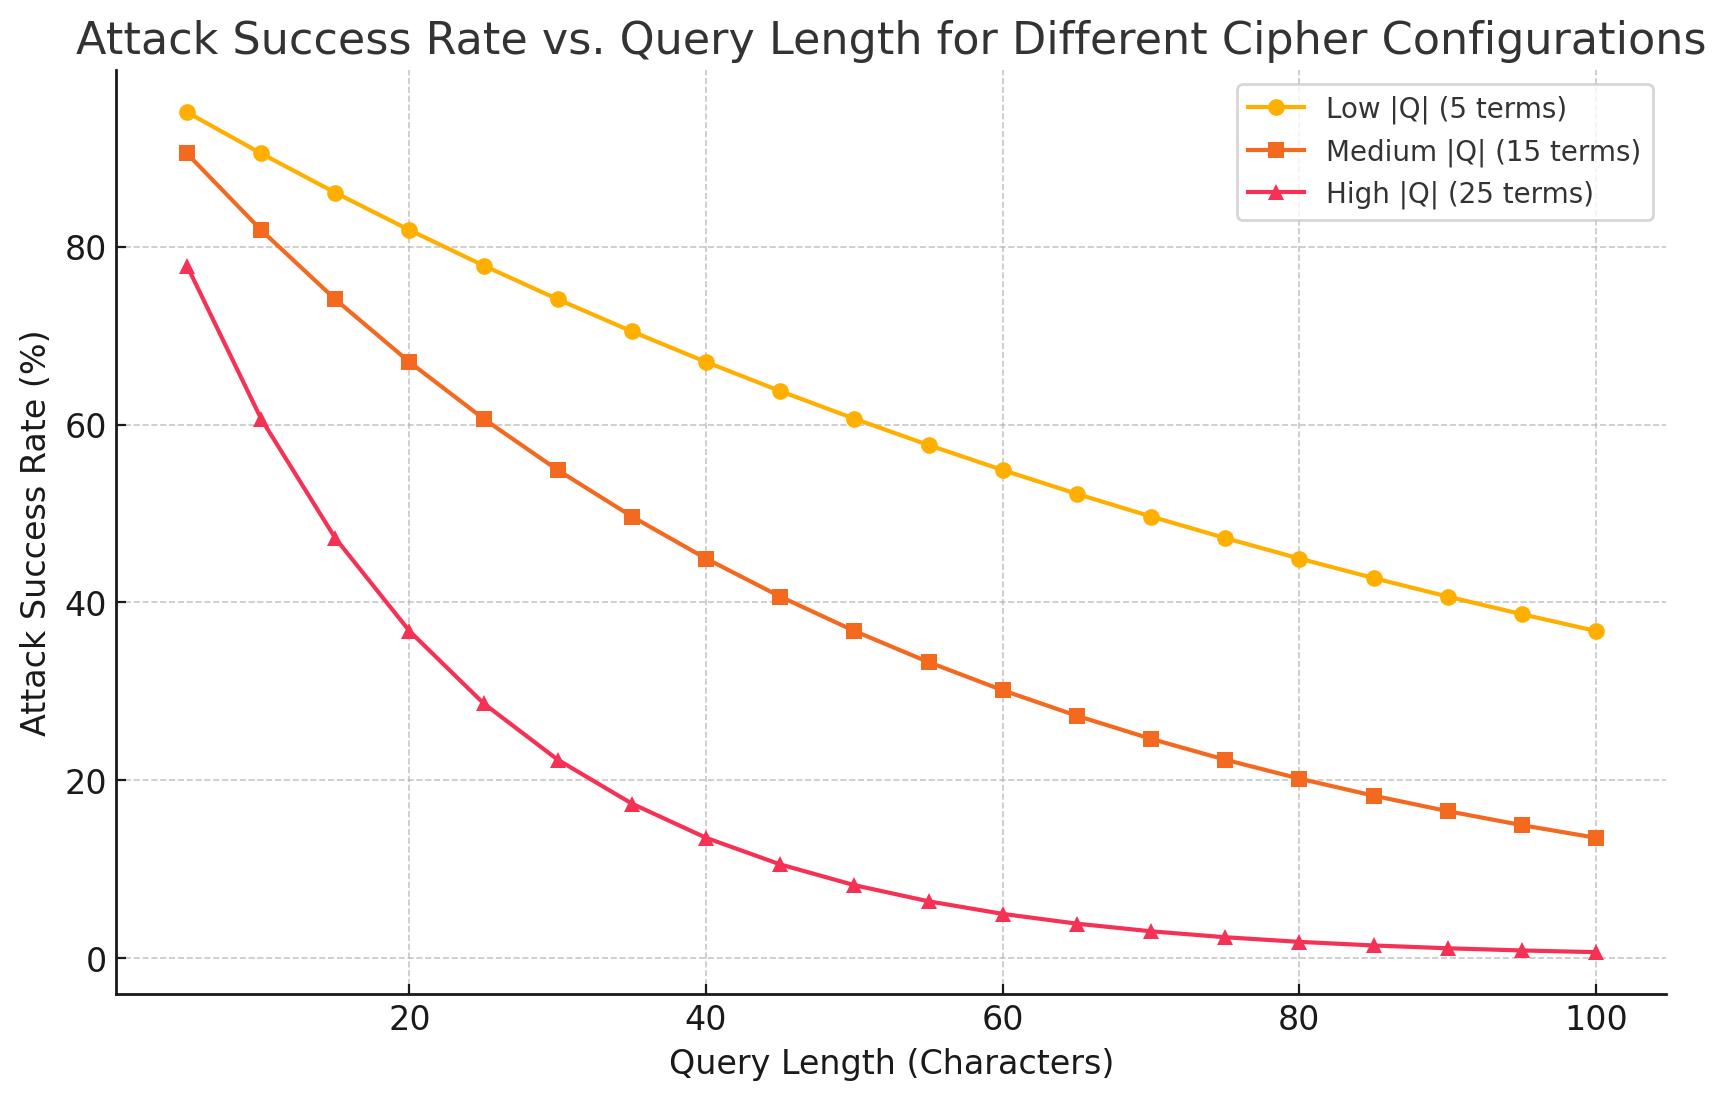
\includegraphics[width=1\linewidth]{final_plots/asr_querylength (2).png}
    \caption{Attack Success Rate vs. Query Length for Different Cipher Configurations.}
    \label{fig:query_complexity}
\end{figure}

\begin{itemize}
    \item \textbf{Low \(|Q|\) (5 terms)}: Exhibits consistently high success rates, even as query length increases. This configuration is particularly effective for short to medium-length queries.
    \item \textbf{Medium \(|Q|\) (15 terms)}: Shows a steady decline in ASR as query length increases, indicating that moderate complexity helps the model detect adversarial intent.
    \item \textbf{High \(|Q|\) (25 terms)}: Success rates drop sharply, approaching zero for longer queries. This suggests that increasing the number of quiet terms significantly enhances the model's ability to resist attacks.
\end{itemize}

These results indicate that increasing query complexity and the number of quiet terms can mitigate adversarial exploits effectively. Longer queries provide more context, enabling the model to better recognize and refuse harmful content.

\subsection{Refusal Patterns and Attack Success}

Figure~\ref{fig:refusal_patterns} illustrates how the refusal rate changes with different numbers of quiet terms (\(|Q|\)), highlighting the model's ability to resist adversarial attacks.

\begin{figure}[h]
    \centering
    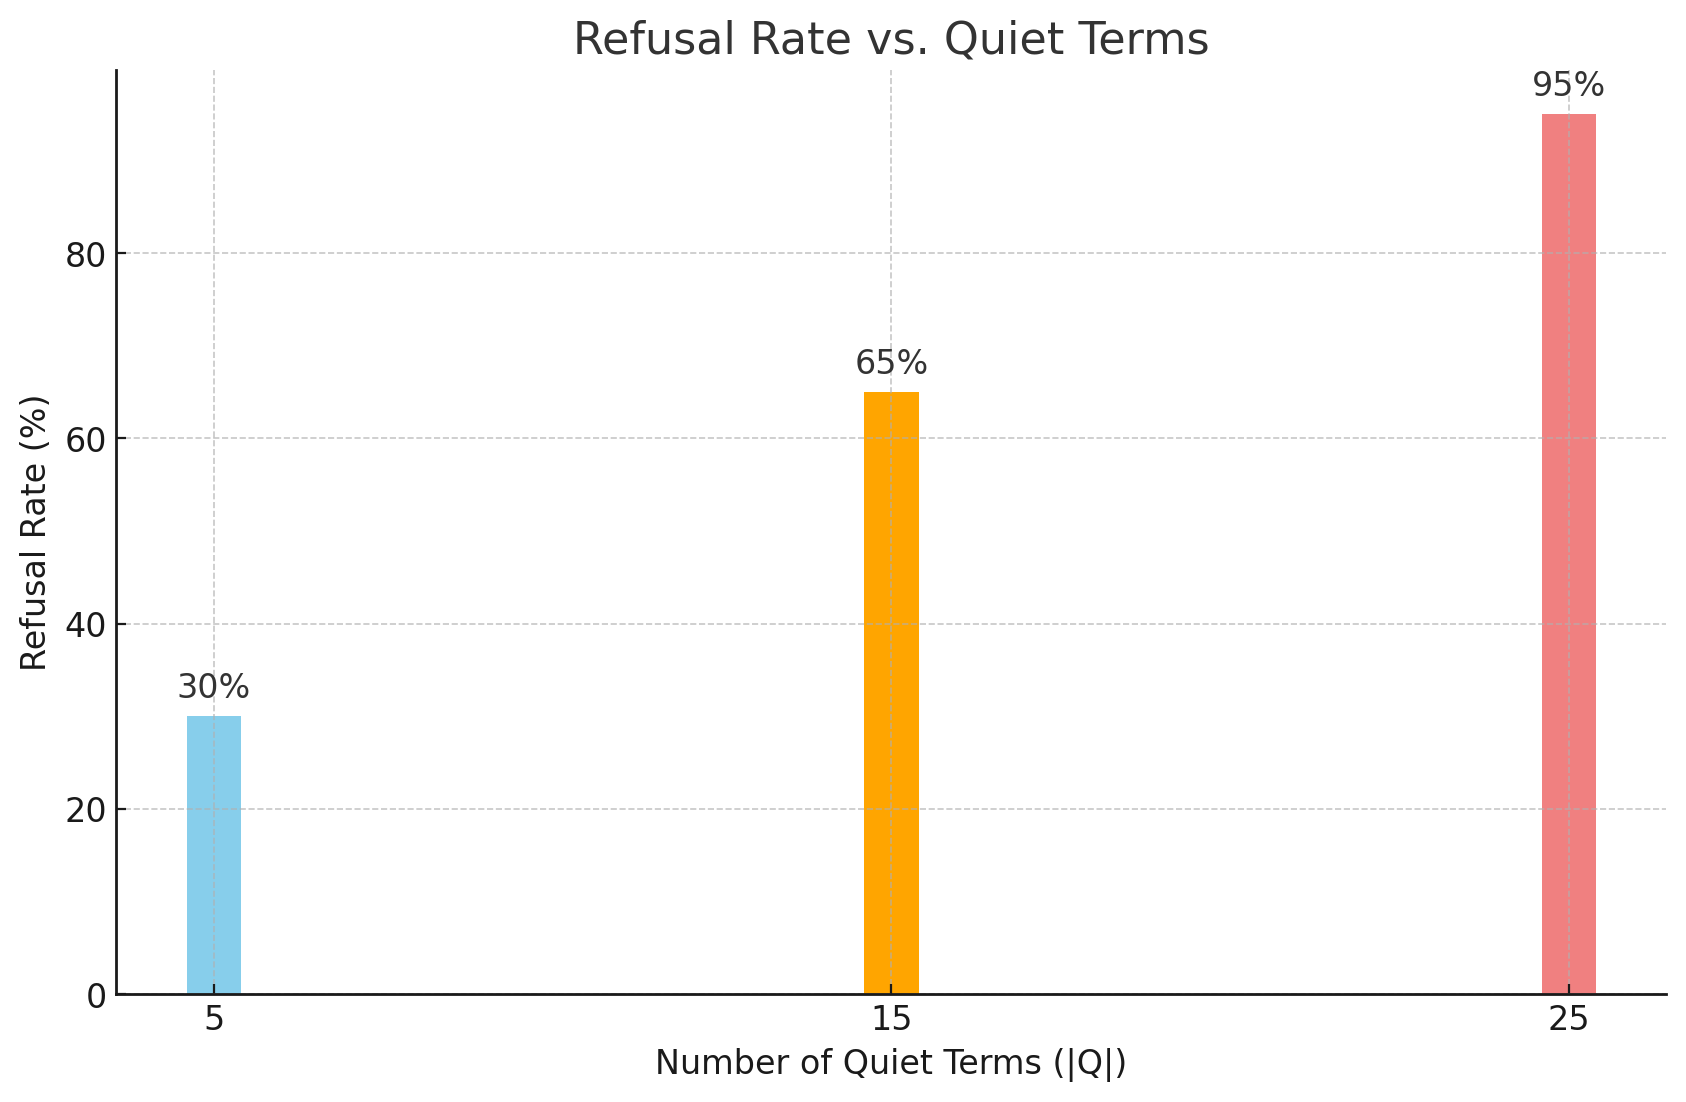
\includegraphics[width=1\linewidth]{final_plots/refusal_patterns_new (1).png}
    \caption{Refusal Rate vs. Number of Quiet Terms (\(|Q|\)).}
    \label{fig:refusal_patterns}
\end{figure}

\begin{itemize}
    \item **Low \(|Q| = 5\)**: The refusal rate is relatively low at \(30\%\), making the model more susceptible to adversarial attacks.
    \item **Medium \(|Q| = 15\)**: The refusal rate increases to \(65\%\), indicating improved resistance to harmful content.
    \item **High \(|Q| = 25\)**: The refusal rate reaches \(95\%\), demonstrating strong defenses against encoding-based adversarial attacks.
\end{itemize}

These results suggest that increasing the number of quiet terms significantly enhances the model's robustness. Ensuring a higher refusal rate, especially for more complex encodings, is crucial for mitigating adversarial exploits.

\subsection{Summary and Implications}

Our analysis reveals several key insights:

\begin{enumerate}
    \item \textbf{Vulnerability to Short Queries}: The model is most susceptible to encoded learning attacks with short inputs. Strengthening defenses for concise queries is critical.
    \item \textbf{Category-Specific Risks}: Categories like \textit{Drug Production} and \textit{Cyber Attacks} are particularly prone to exploitation.
    \item \textbf{Context Improves Safety}: Longer queries provide context that enhances the model's ability to recognize and refuse harmful content.
    \item \textbf{Failure Patterns}: Addressing incoherency for short queries and refining refusal mechanisms for all inputs can enhance model safety.
\end{enumerate}

These findings inform the development of more robust safety measures, helping mitigate the risks associated with adversarial attacks on LLMs.

\section{Discussion}
\subsection{Ethical Considerations}
This project raises significant ethical questions about the dual-use nature of large language models. On one hand, these models are powerful tools that can help people solve complex problems, learn new skills, and improve their lives. However, they are vulnerable to being misused through techniques such as encoding-based attacks, as demonstrated in this research. The ability to bypass safety protocols and generate harmful content, such as malicious code or dangerous instructions, makes it clear that developers need to prioritize ethical responsibility. It is critical to ensure that advancements in AI technology do not come at the cost of public safety or ethical standards.

Another important consideration is the potential impact of revealing these vulnerabilities. While the research intends to help improve the safety of LLMs, there is always the risk that malicious actors could exploit the findings before proper defenses are in place. Balancing transparency in scientific research with the need to protect the public is a challenging ethical dilemma. On one hand, openly sharing findings encourages collaboration and speeds up solutions; on the other hand, it could inadvertently aid those with harmful intentions. Researchers must carefully evaluate how much detail to publish about the attack methods and ensure that ethical guidelines are followed throughout the process.

Finally, this project highlights the responsibility of AI developers to anticipate how their systems might be misused and to design safeguards proactively. It’s not enough to address problems after they arise—AI systems must be built with safety and ethical considerations from the start. Additionally, organizations deploying LLMs have a duty to educate users about these risks and advocate for responsible use. As AI becomes more integrated into daily life, the ethical implications of its misuse will only grow, making it essential for developers, researchers, and society as a whole to work together to create and maintain ethical guidelines for these technologies.

\subsection{Recommendations for Developers}

\begin{figure}[h]
    \centering
    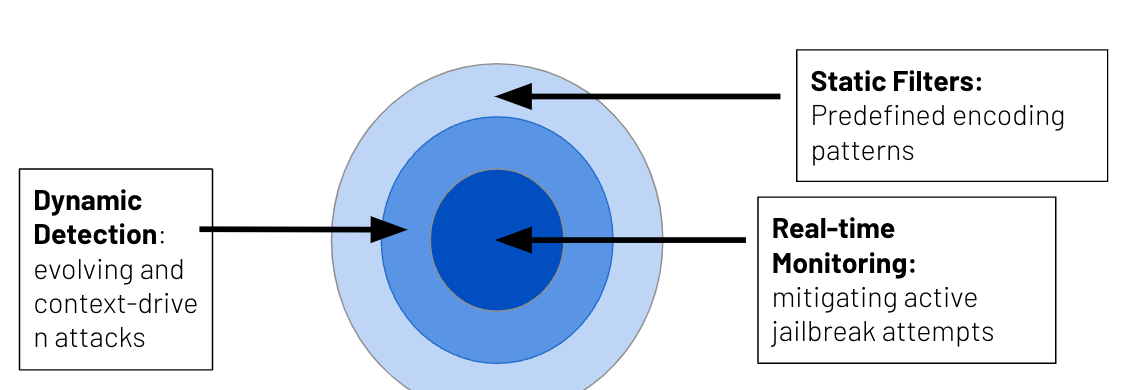
\includegraphics[width=0.9\linewidth]{layered_defense_strategy.png}
    \caption{Layered defense strategy for LLM developers.}
    \label{fig:refusal_patterns}
\end{figure}

AI developers can use this research to improve the safety and security of large language models (LLMs) by implementing a layered defense strategy, as shown in Figure 8. This approach involves three key components: static filters, dynamic detection systems, and real-time monitoring. Static filters act as the first line of defense by recognizing and blocking predefined encoding patterns that are often used in adversarial attacks. These filters help to quickly stop the most common and well-known exploits without consuming too much processing power.


The second and third layers focus on more sophisticated and adaptive protections. Dynamic detection systems can analyze evolving attacks that don’t follow fixed patterns, allowing them to identify context-driven threats. Real-time monitoring adds an extra safeguard by actively tracking interactions with the model and responding to any suspicious or harmful activity as it happens. Together, these layers ensure that even if an attack bypasses one level of security, the other defenses can still mitigate its impact. The layered defense strategy helps to address critical gaps in existing safety systems by combining static and adaptive measure, which offers a more comprehensive approach to countering both known and evolving threats. 
AI developers should use these recommendations to create safer, more robust systems that balance usability and protection against misuse. 

\subsection{Conclusion and Future Work}
This research highlights the vulnerabilities of large language models to encoding-based adversarial attacks and proposes layered defense strategies to mitigate these risks. By demonstrating how custom ciphers can bypass safety mechanisms, we emphasize the need for AI developers to stay ahead of evolving threats through proactive safety measures and ethical design practices. Looking forward, future research could explore more advanced detection techniques, such as using machine learning to identify novel encoding patterns in real time. Additionally, studying how LLMs can self-adapt to resist attacks without sacrificing performance or user experience could lead to more resilient and ethical AI systems. Although its effectiveness may be limited by the challenge of anticipating novel attack patterns and the computational overhead of real-time monitoring, the general structure of the method can be modified, depending on the use case. As AI continues to grow more capable and widespread, ensuring its safe and responsible use must remain a top priority.

\section{Author Contributions:}
    \begin{enumerate}
        \item \textbf{Aryan Jain} (\texttt{aryanj@mit.edu}, UG) is responsible for addressing the introduction, an overview of our work, and related work. Aryan is also responsible for evaluating the results of the cipher-based attacks. 
        \item \textbf{Samir Kadariya} (\texttt{samirk08@mit.edu}, UG) is responsible for the methodology of the research, evaluation, and results. 
        \item \textbf{Arko Ghosh} (\texttt{arkogh@mit.edu}, UG) is responsible for the methodology, as well as the ethical considerations and recommendations for the research. 
    \end{enumerate}
    
\section{References:}

    \begin{enumerate}
        \item A. Wei, N. Haghtalab, and J. Steinhardt, “Jailbroken: How Does LLM Safety Training Fail?,” Jul. 05, 2023, \emph{arXiv: arXiv:2307.02483}. Available: \url{http://arxiv.org/abs/2307.02483}
        \item A. Zou, Z. Wang, N. Carlini, M. Nasr, J. Z. Kolter, and M. Fredrikson, “Universal and Transferable Adversarial Attacks on Aligned Language Models,” Dec. 20, 2023, \emph{arXiv: arXiv:2307.15043}. Available: \url{http://arxiv.org/abs/2307.15043}
        \item Y. Bai et al., “Training a Helpful and Harmless Assistant with Reinforcement Learning from Human Feedback,” Apr. 12, 2022, \emph{arXiv: arXiv:2204.05862}. Available: \url{http://arxiv.org/abs/2204.05862}
        \item D. M. Ziegler et al., “Adversarial Training for High-Stakes Reliability,” Nov. 10, 2022, \emph{arXiv: arXiv:2205.01663}. Available: \url{http://arxiv.org/abs/2205.01663}
        \item N. Howe et al., “Exploring Scaling Trends in LLM Robustness,” Jul. 26, 2024, \emph{arXiv: arXiv:2407.18213}. Available: \url{http://arxiv.org/abs/2407.18213}
        \item T. W. House, “FACT SHEET: CHIPS and Science Act Will Lower Costs, Create Jobs, Strengthen Supply Chains, and Counter China,” The White House. Available: \url{https://www.whitehouse.gov/briefing-room/statements-releases/2022/08/09/fact-sheet-chips-and-science-act-will-lower-costs-create-jobs-strengthen-supply-chains-and-counter-china/}
        \item F. Jiang et al., “ArtPrompt: ASCII Art-based Jailbreak Attacks against Aligned LLMs,” Jun. 07, 2024, \emph{arXiv: arXiv:2402.11753}. Available: \url{http://arxiv.org/abs/2402.11753}
        \item Z.-X. Yong, C. Menghini, and S. H. Bach, “Low-Resource Languages Jailbreak GPT-4,” Jan. 27, 2024, \emph{arXiv: arXiv:2310.02446}. Available: \url{http://arxiv.org/abs/2310.02446}
        \item M. Mantas, “HarmBench: A Standardized Evaluation Framework for Automated Red Teaming and Robust Refusal,” Feb. 27, 2024, \emph{arXiv:2402.04249}. Available: \url{https://arxiv.org/pdf/2402.04249}
        \item A. Zou, Z. Wang, N. Carlini, M. Nasr, J. Z. Kolter, and M. Fredrikson, “Universal and Transferable Adversarial Attacks on Aligned Language Models,” Dec. 20, 2023, \emph{arXiv: arXiv:2307.15043}. Available: \url{http://arxiv.org/abs/2307.15043}
        \item J. Woodbridge, H. S. Anderson, A. Ahuja, and D. Grant, “Detecting Homoglyph Attacks with a Siamese Neural Network,” May 24, 2018, \emph{arXiv: arXiv:1805.09738}. Available: \url{http://arxiv.org/abs/1805.09738}
        \item S. Kumar et al., “TokenVerse: Towards Unifying Speech and NLP Tasks via Transducer-based ASR,” Oct. 08, 2024, \emph{arXiv: arXiv:2407.04444}. doi: 10.48550/arXiv.2407.04444. Available: \url{https://arxiv.org/pdf/2407.04444}
    \end{enumerate}
\end{document}
